\documentclass[a4paper,11pt]{article}
\usepackage[T1]{fontenc}
\usepackage[toc,page]{appendix}
\usepackage[utf8]{inputenc}
\usepackage{lmodern}
\usepackage{listings}
\usepackage{verbatim}
\usepackage{multicol}
\usepackage{csquotes}
\usepackage{fancyhdr}
\usepackage{longtable}
\usepackage{color}
\usepackage{amsmath}
\usepackage{natded}
\usepackage{graphicx}
\usepackage{fancyvrb}
\usepackage{amssymb}
\usepackage{wrapfig}
% include code listing options
% define colors for code listings
\definecolor{mygreen}{rgb}{0,0.6,0}
\definecolor{mygray}{rgb}{0.5,0.5,0.5}
\definecolor{mymauve}{rgb}{0.58,0,0.82}

% define options for code listings
\lstset{ %
  backgroundcolor=\color{white},   % choose the background color; you must add \usepackage{color} or \usepackage{xcolor}
  basicstyle=\footnotesize,        % the size of the fonts that are used for the code
  breakatwhitespace=false,         % sets if automatic breaks should only happen at whitespace
  breaklines=true,                 % sets automatic line breaking
  captionpos=b,                    % sets the caption-position to bottom
  commentstyle=\color{mygreen},    % comment style
  deletekeywords={...},            % if you want to delete keywords from the given language
  escapeinside={\%*}{*)},          % if you want to add LaTeX within your code
  extendedchars=true,              % lets you use non-ASCII characters; for 8-bits encodings only, does not work with UTF-8
  frame=single,                    % adds a frame around the code
  keepspaces=true,                 % keeps spaces in text, useful for keeping indentation of code (possibly needs columns=flexible)
  keywordstyle=\color{blue},       % keyword style
  language=Prolog,                 % the language of the code
  morekeywords={*,...},            % if you want to add more keywords to the set
  numbers=left,                    % where to put the line-numbers; possible values are (none, left, right)
  numbersep=5pt,                   % how far the line-numbers are from the code
  numberstyle=\tiny\color{mygray}, % the style that is used for the line-numbers
  rulecolor=\color{black},         % if not set, the frame-color may be changed on line-breaks within not-black text (e.g. comments (green here))
  showspaces=false,                % show spaces everywhere adding particular underscores; it overrides 'showstringspaces'
  showstringspaces=false,          % underline spaces within strings only
  showtabs=false,                  % show tabs within strings adding particular underscores
  stepnumber=1,                    % the step between two line-numbers. If it's 1, each line will be numbered
  stringstyle=\color{mymauve},     % string literal style
  tabsize=2,                       % sets default tabsize to 2 spaces
  title=\lstname                   % show the filename of files included with \lstinputlisting; also try caption instead of title
}

\newcounter{question}
\setcounter{question}{0}

\title{Labb 2 \\ Logic for computer science}
\author{
  {\bf Christopher Lillthors}\\
  \textbf{911005-3817} \\\\
  {\bf Viktor Kronvall}\\
  \textbf{920225-5478}\\
  \\
  Kurskod: DD1350\\
  %Ev gruppnummer\\
  KTH -- HT14\\
  lillt@kth.se\\
  vkr@kth.se
}

\pagestyle{fancy}
\setlength{\headheight}{54pt}
\fancyfoot[C,R]{\thepage}
\fancyfoot[C]{}
\rhead{\textbf{Labb 2 -- Lillthors \& Kronvall} \\ \date{\today} \\ \ \\}
\lhead{\textbf{Royal Institute of Technology} \\ School of Computer science and communication \\ Civilingenjörsprogrammet Datateknik}
\setlength{\parindent}{0in}
\setlength{\parskip}{0.1in}
\date{\today}
\begin{document}

%Include the Q&A commands
\newcommand\Que[1]{%
   \leavevmode\par
   \stepcounter{question}
   \noindent
   \thequestion. Q --- #1\par}

\newcommand\Ans[2][]{%
    \leavevmode\par\noindent
   {\leftskip37pt
    A --- \textbf{#1}#2\par}}

\maketitle
\thispagestyle{empty}
\begin{abstract}

This paper describes a simple model verification system written in the programming language Prolog.
The system can verify models for a variety of rules given that the input is written using CTL.
\end{abstract}
\renewcommand{\arraystretch}{1.2}
\newpage
\thispagestyle{empty}
\tableofcontents
\newpage
\clearpage
\setcounter{page}{1}

\section{Background}

\newpage

\section{Example model}
We construct a model $\mathcal{M}$ for a web client that is accessing a server which requires authentication and authorization
before some of the resources hosted by the server may be accessed.
\begin{figure}[ht]
\caption{Graph of the model}
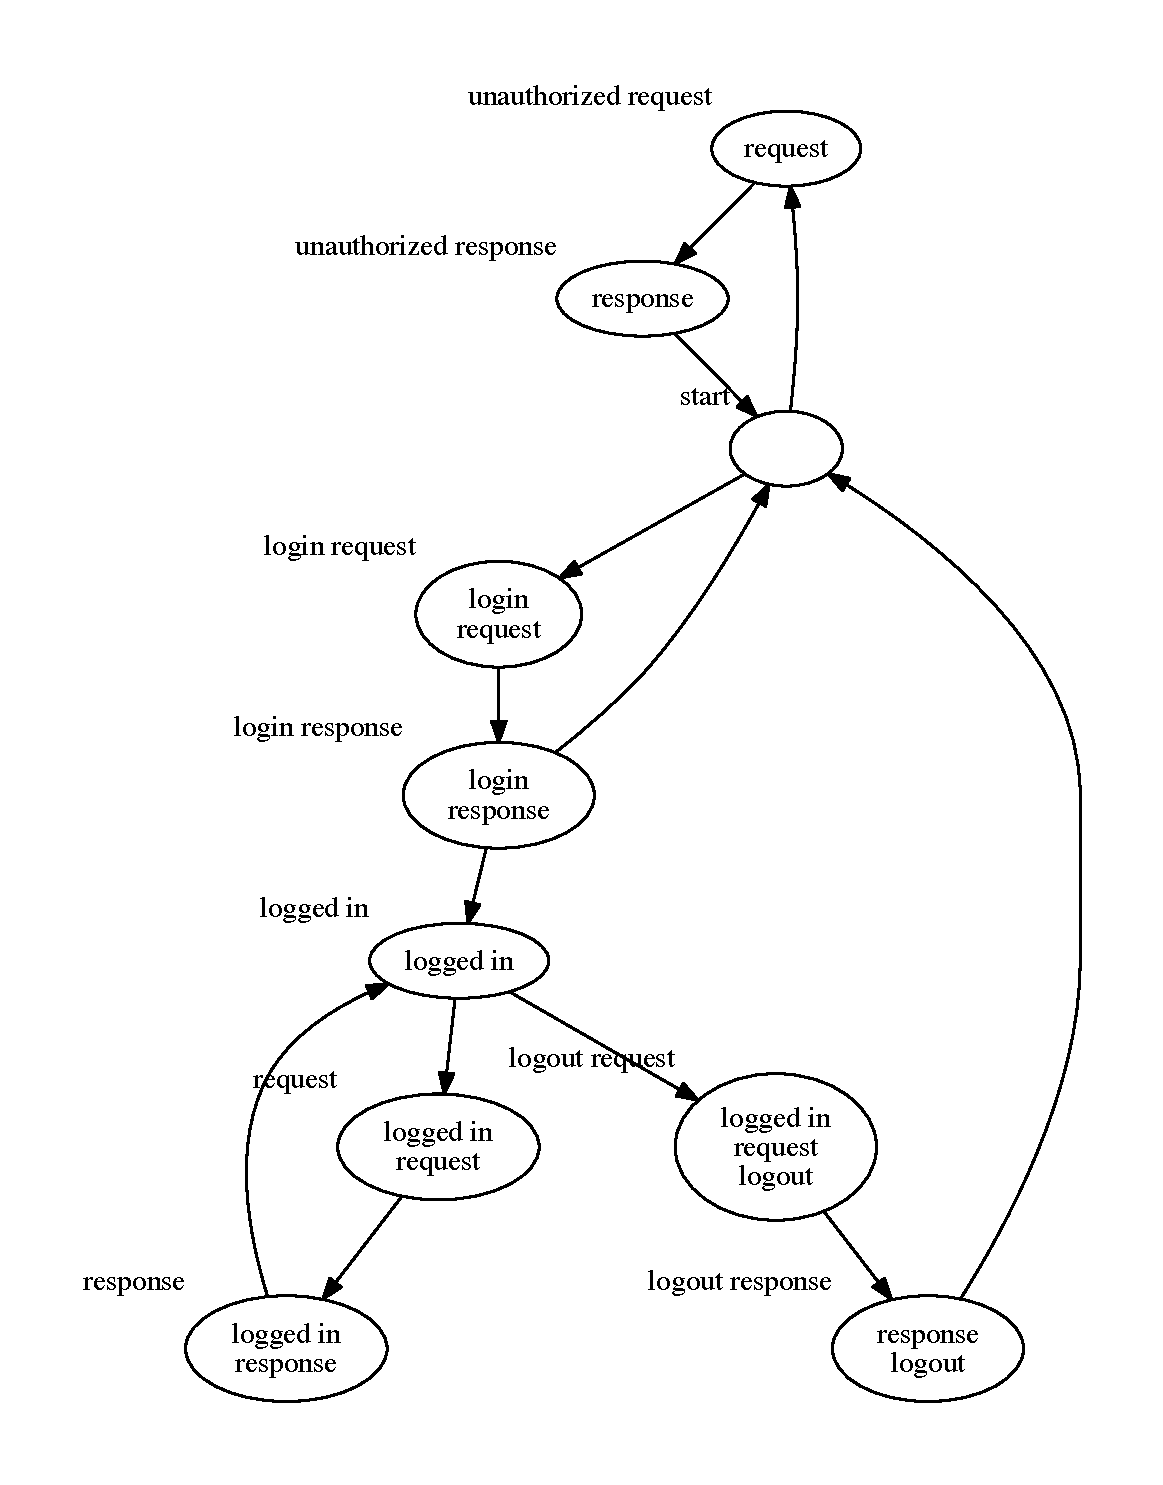
\includegraphics[scale=0.6]{model.pdf}
\label{fig:graph}
\end{figure}

\newpage
\subsection{Valid assumption}
Given the state \textit{logged in} assume that $EF(\neg logged \: in)$ holds.

This formula describes the condition that given a logged in state, there is a path
to reach a state where one is not logged in.

By analyzing the graph in figure \ref{fig:graph} we can see that one possible state that is reachable from
\textit{logged in} is the state \textit{start} where one is not logged in. Therefore we can conclude that this is intuitively correct.

\subsection{Invalid assumption}
Given the state \textit{login response} assume that $AX(logged \: in)$ holds.

This formula describes the condition that given a login response state, the next state must contain the propositional variable \textit{logged in}, i.e $L(s)=logged \: in$.

By analyzing the graph in figure \ref{fig:graph} and looking at the paths from \textit{login response} there is one path that describes a failed login where one is sent back to the \textit{start} state. Given this we deduce that the assumption does not hold as $logged \: in \notin L(start)$.

\section{Implementation}

\section{Results}
All the given tests are passing.

\section{Questions}

\Que{What's the difference between your implementation and the implementation written in the text book?}
%TODO
\Ans{
  contradictions
  until
  implications
}

\Que{How did you handle a variable number of premises in rules?}
\Ans{We use the built in predicate \textit{member} to iterate over all the neighbors.}

\Que{How big models can you handle with your implementation?}
\Ans{The time complexity $\mathcal{O}(n^p)$ increases by a factor for each time a rule that is using all neighbors to a state. That means that $p$ is increased by one for each time and we quickly approach a cubic asymptotic progression of the time $\mathcal{O}(n^3)$. This leads to an untenable situation for solving formulas in a reasonable amount of time for bigger models. For example, a model that has $10^3$ neighbors for each state, progressing only three states from the starting state will result in over $10^9$ checks being performed.}

% \mathcal{p} \fraq{-}{}p \in L(s)

\newpage
\begin{appendices}
\section{Source code}
\lstinputlisting{labb2.pl}
\section{Valid assumption}
\verbatiminput{valid_model.txt}
\section{Invalid assumption}
\verbatiminput{invalid_model.txt}
\end{appendices}
\end{document}